\section{Results}

\subsection{Baseline Results on CTFTiny}
To establish a baseline for large language models (LLMs) on the \texttt{CTFTiny} benchmark, we evaluated seven state-of-the-art models across multiple cybersecurity domains. Among them, Claude 4 Sonnet achieved the highest performance, solving 38 out of 50 challenges for a 76\% success rate. Gemini 2.5 Flash followed with 32 correct solutions (64\%), while Gemini 2.5 Pro and GPT‑4.1 completed 24 (48\%) and 20 (40\%) challenges, respectively. The remaining models demonstrated more limited capabilities: Qwen 3 solved 14 challenges (28\%), DeepSeek V3 solved 11 (22\%), and LLaMA 4 Maverick 17B completed only 4 (8\%).


\begin{figure}[htbp]
    \centering
    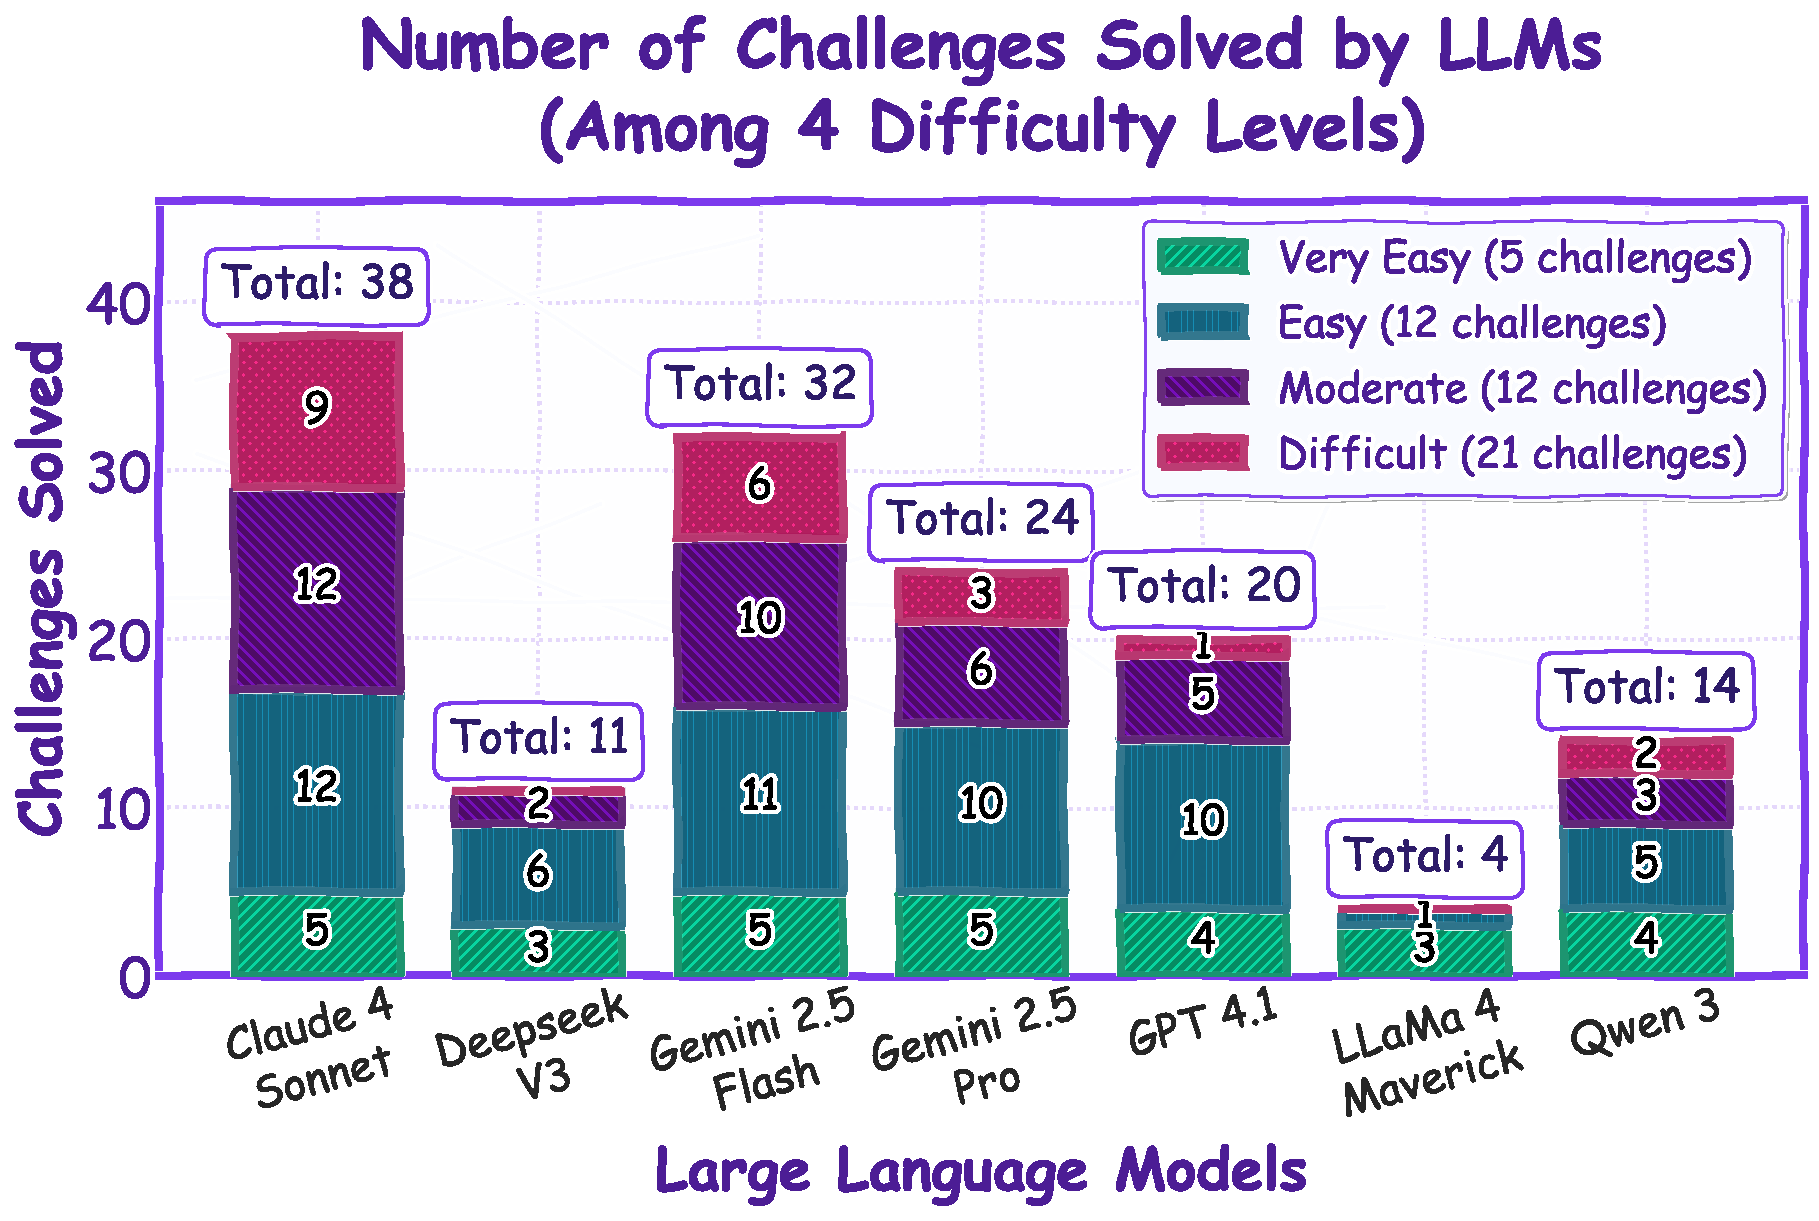
\includegraphics[width=\linewidth]{diagrams/difficulty_solution.pdf}
    \caption{Challenge solves by model and difficulty, showing sharp performance drops as complexity rises.}
    \label{fig:stat_diff}
\end{figure}

Figure~\ref{fig:stat_diff} breaks down each model’s solved challenges into four difficulty bands (\emph{very easy}, \emph{easy}, \emph{medium}, \emph{difficult}), as described in Section~\ref{sec:ctftiny}. Top models maintain near-perfect scores on the simplest challenges but decline sharply as complexity rises. Claude 4 Sonnet and Gemini 2.5 Flash solve 100\% \emph{very easy} instances and achieve over 40\% and 25\% respectively on \emph{difficult} challenges, underscoring their robustness across task difficulty. Mid-ranked models (GPT-4.1, Qwen 3) have reasonable accuracy on \emph{easy} tasks but fall below 50\% in the \emph{medium} band and solve less than 10\% \emph{difficult} challenges. Lower-ranked models (DeepSeek V3, LLaMA 4 Maverick 17B) succeed only on \emph{very easy} and a  fraction of \emph{easy} problems. This highlights performance gaps on difficult CTFs  underscoring the need for robust reasoning and decomposition strategies in agent designs.

\begin{table}[!b]
    \centering
    \small
    \setlength{\tabcolsep}{4pt}
    \caption{Model performance on \texttt{CTFTiny}, with Claude 4 Sonnet leading but domain strengths varying.}
    \label{tab:ctftiny-percentage-corrected}
    \begin{tabular}{lccccccc}
    \toprule
    \textbf{Metric} & \rotatebox{90}{\textbf{Claude4S}} & \rotatebox{90}{\textbf{DeepSeekV3}} & \rotatebox{90}{\textbf{Gemini2.5F}} & \rotatebox{90}{\textbf{Gemini2.5P}} & \rotatebox{90}{\textbf{GPT 4.1}} & \rotatebox{90}{\textbf{LLaMa 4M}} & \rotatebox{90}{\textbf{Qwen 3}} \\
    \midrule
    Total (\%) & \textbf{76} & 22 & 64 & 48 & 40 & 8 & 28 \\
    Cost (\$) & 1.16 & \textbf{0.02} & 0.26 & 0.33 & 0.77 & 0.14 & \textbf{0.04} \\
    Cry (\%) & \textbf{75.0} & 16.7 & 50.0 & 50.0 & 33.3 & 0.0 & 25.0 \\
    For (\%) & 50.0 & 0.0 & \textbf{100.0} & \textbf{100.0} & 0.0 & 0.0 & 0.0 \\
    Pwn (\%) & 63.6 & 18.2 & \textbf{72.7} & 45.5 & 36.4 & 0.0 & 18.2 \\
    Rev (\%) & \textbf{81.3} & 18.8 & 68.8 & 37.5 & 37.5 & 12.5 & 18.8 \\
    Web (\%) & \textbf{100.0} & 66.7 & 33.3 & 33.3 & 66.7 & 33.3 & \textbf{100.0} \\
    Misc (\%) & \textbf{83.3} & 33.3 & 66.7 & 66.7 & 66.7 & 16.7 & 50.0 \\
    \bottomrule
    \label{tab:baseline}
    \end{tabular}
\end{table}

A category-level analysis reveals pronounced differences in model strengths and specialization. In \emph{reverse engineering}, Claude 4 Sonnet leads with an 81.3\% success rate (13/16), followed by Gemini 2.5 Flash at 68.8\%. In \emph{cryptography}, Claude 4 Sonnet once again tops the leaderboard with 75\% (9/12), while both Gemini variants reach 50\%. Notably, Gemini 2.5 Flash outperforms Claude 4 Sonnet in \emph{binary exploitation}, achieving 72.7\% versus 63.6\%, indicating a clear domain-specific specialization. \emph{Forensics} tasks yield perfect scores from both Gemini models, though the sample size remains small. In \emph{web} exploitation, Claude 4 Sonnet and Qwen 3 both achieve 100\%. Finally, in the \emph{miscellaneous} category, Claude 4 Sonnet maintains its overall lead at 83.3\%.
By mapping performance across difficulty tiers and categories, \texttt{CTFTiny} transforms raw scores into diagnostic insights, revealing each model’s unique strengths and blind spots, and charting an informed path toward resilient AI agents for cybersecurity.

\subsection{CTF Competency Index (CCI)}

Figure~\ref{fig:cci} presents the CTF Competency Index distribution for each model on the \texttt{CTFTiny} baseline. Claude 4 Sonnet consistently leads across all skill dimensions, with CCI from 77.5 to 84.5, reflecting robust reasoning and adaptability even on harder tasks. Gemini 2.5 Pro also delivers strong, balanced scores, especially in exploitation and adaptability, while Gemini 2.5 Flash, despite more solves, yields a lower overall CCI due to less systematic approaches. GPT-4.1 shows moderate results, particularly lagging in efficiency and adaptability. Qwen 3 performs reasonably on core skills but is limited by weak efficiency and adaptability. DeepSeek V3 and LLaMA 4 Maverick 17B stay at the lower end, underscoring persistent struggles, even on easy tasks.

\begin{figure}[!t]
\hspace*{-0.15in}
    \centering
    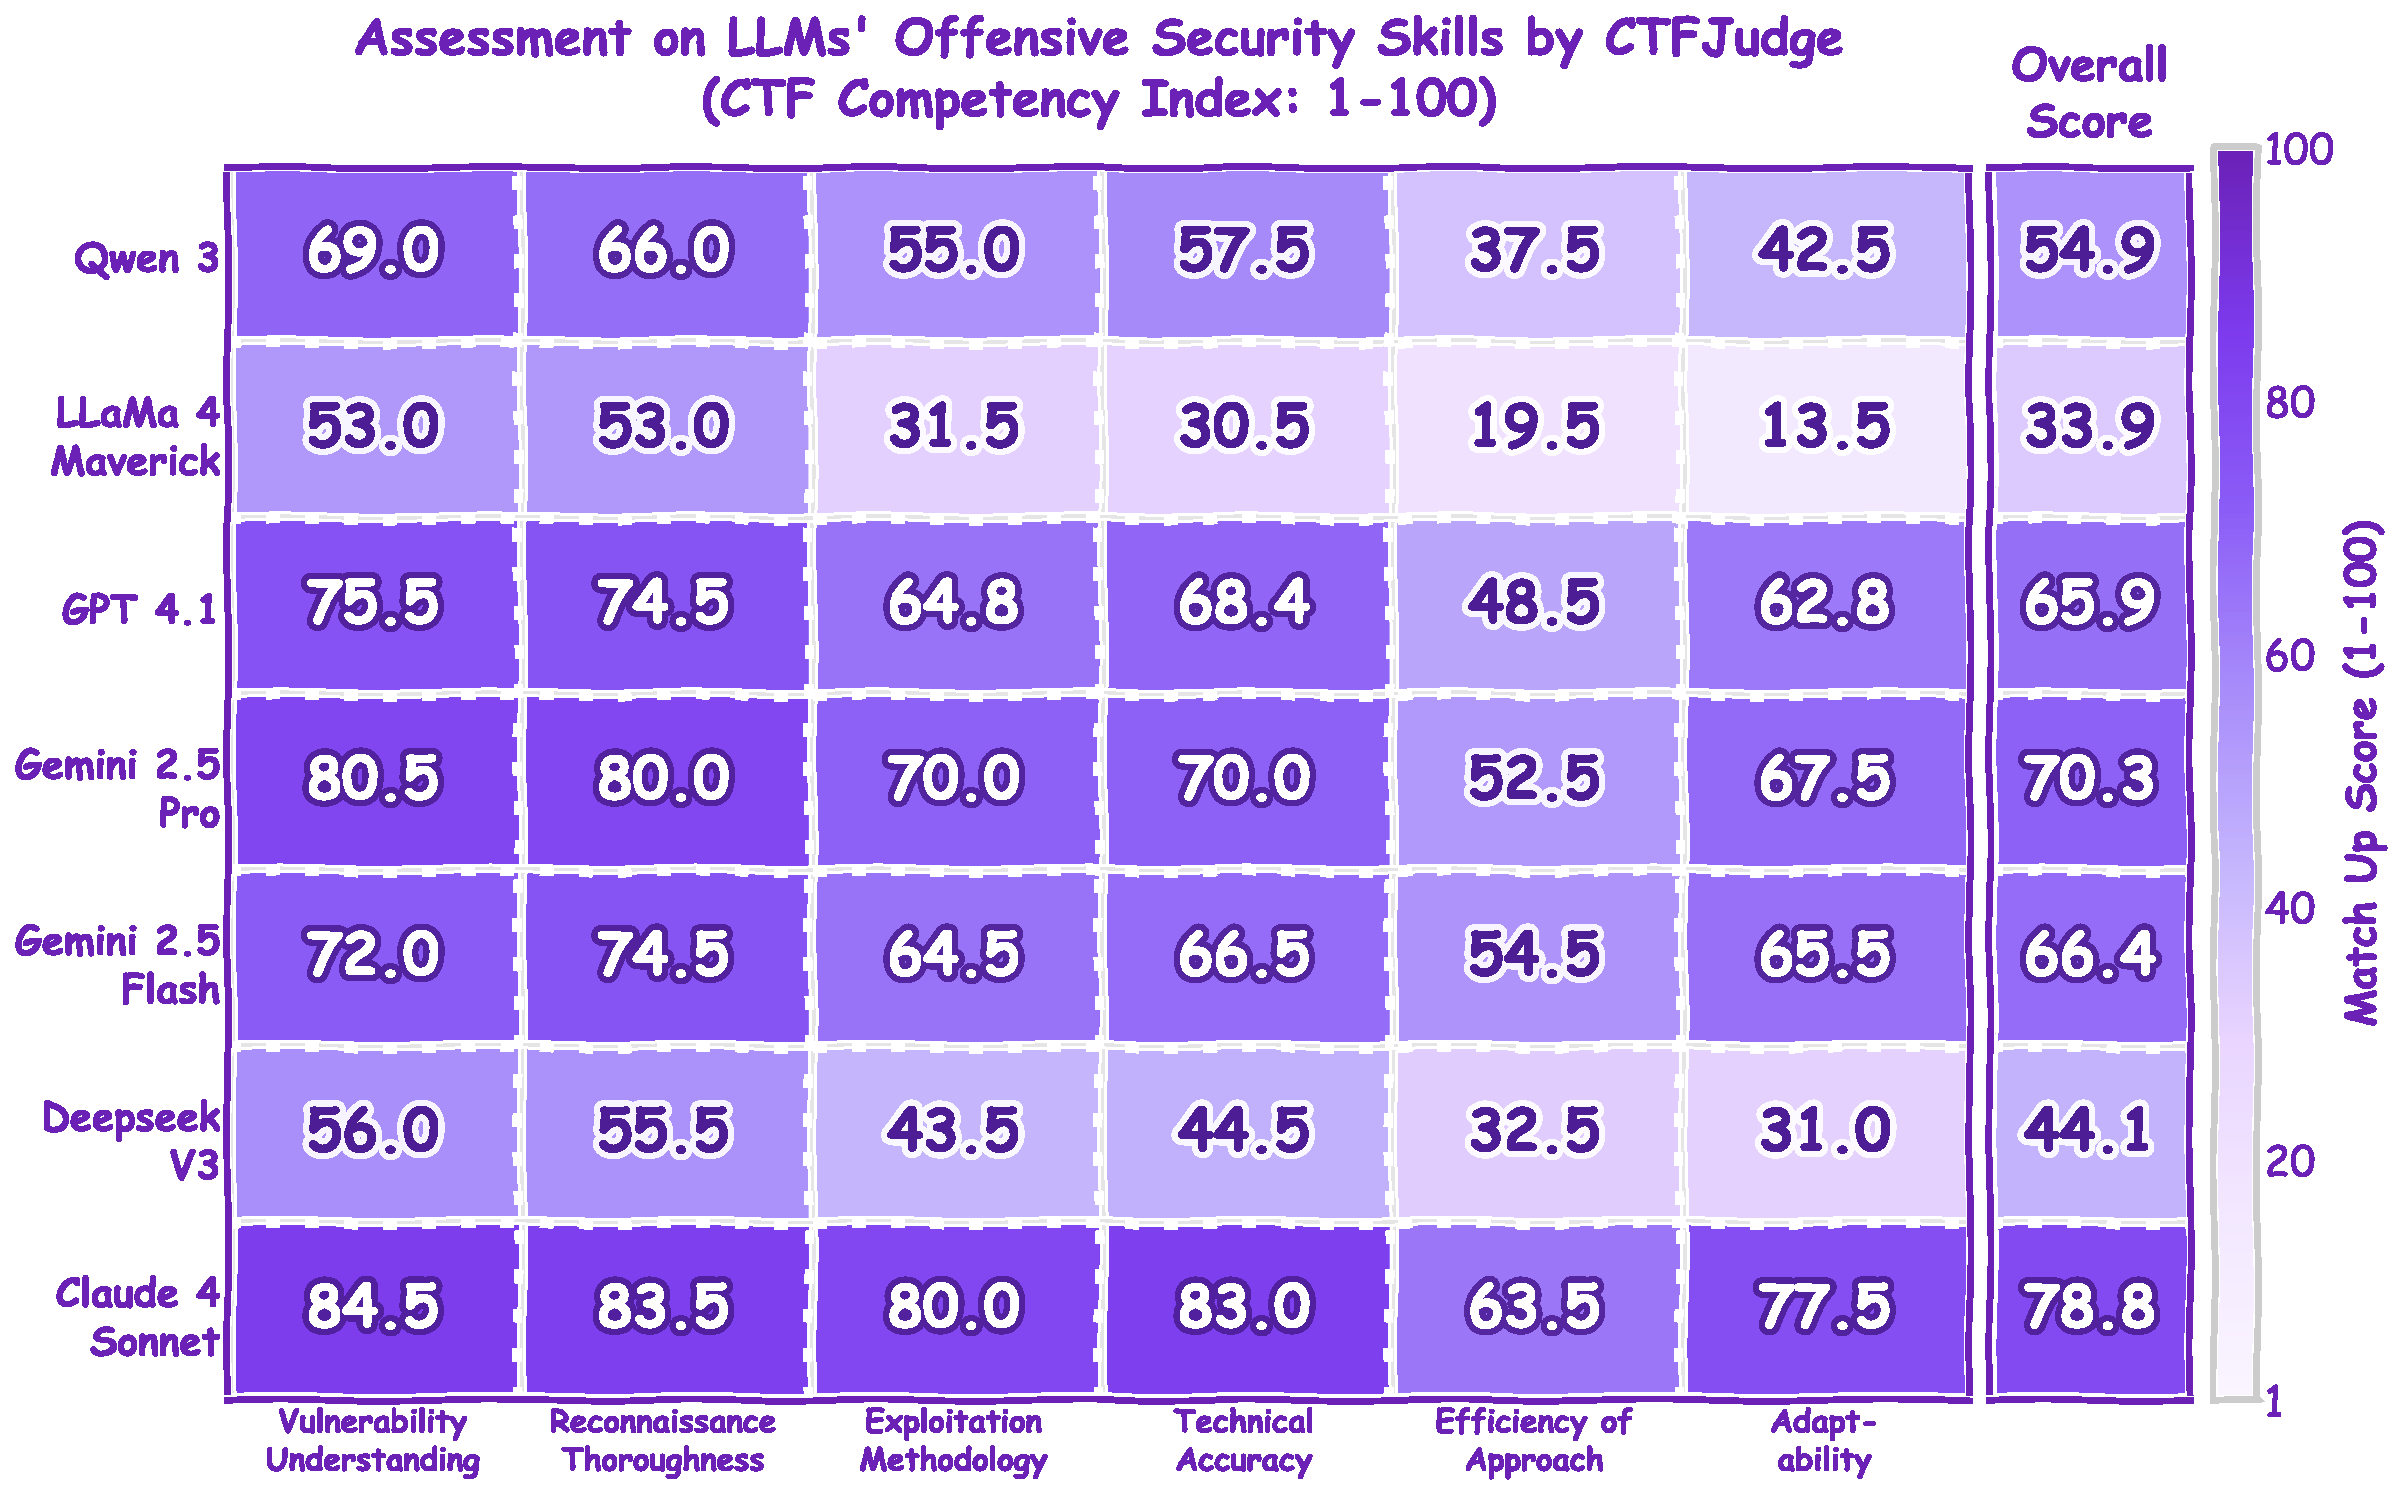
\includegraphics[width=1.1\linewidth]{diagrams/ctfjudge_result.pdf}
    \caption{CTF Competency Index by model.} %, high solve rates don’t always mean better reasoning.}
    \label{fig:cci}
\end{figure}

Figures~\ref{fig:cci_succ} and \ref{fig:cci_fail} show CCI cleanly separating outcomes: successes cluster at high, uniform scores; failures sit mid–low with sharp dips. Claude 4 and Gemini Pro/Flash lead; GPT-4.1/Qwen 3 are mid; DeepSeek/LLaMA weak. Reconnaissance and Vulnerability Understanding change little across outcomes. The separation comes from Exploitation Methodology, Efficiency of Approach, and Adaptability, which drop sharply on failed runs. Successful trajectories also show lower variance across skills, indicating steadier end-to-end execution. Thus, CCI not only distinguishes success from failure but also pinpoints where the pipeline breaks.

\begin{figure}[htbp]
\hspace*{-0.15in}
    \centering
    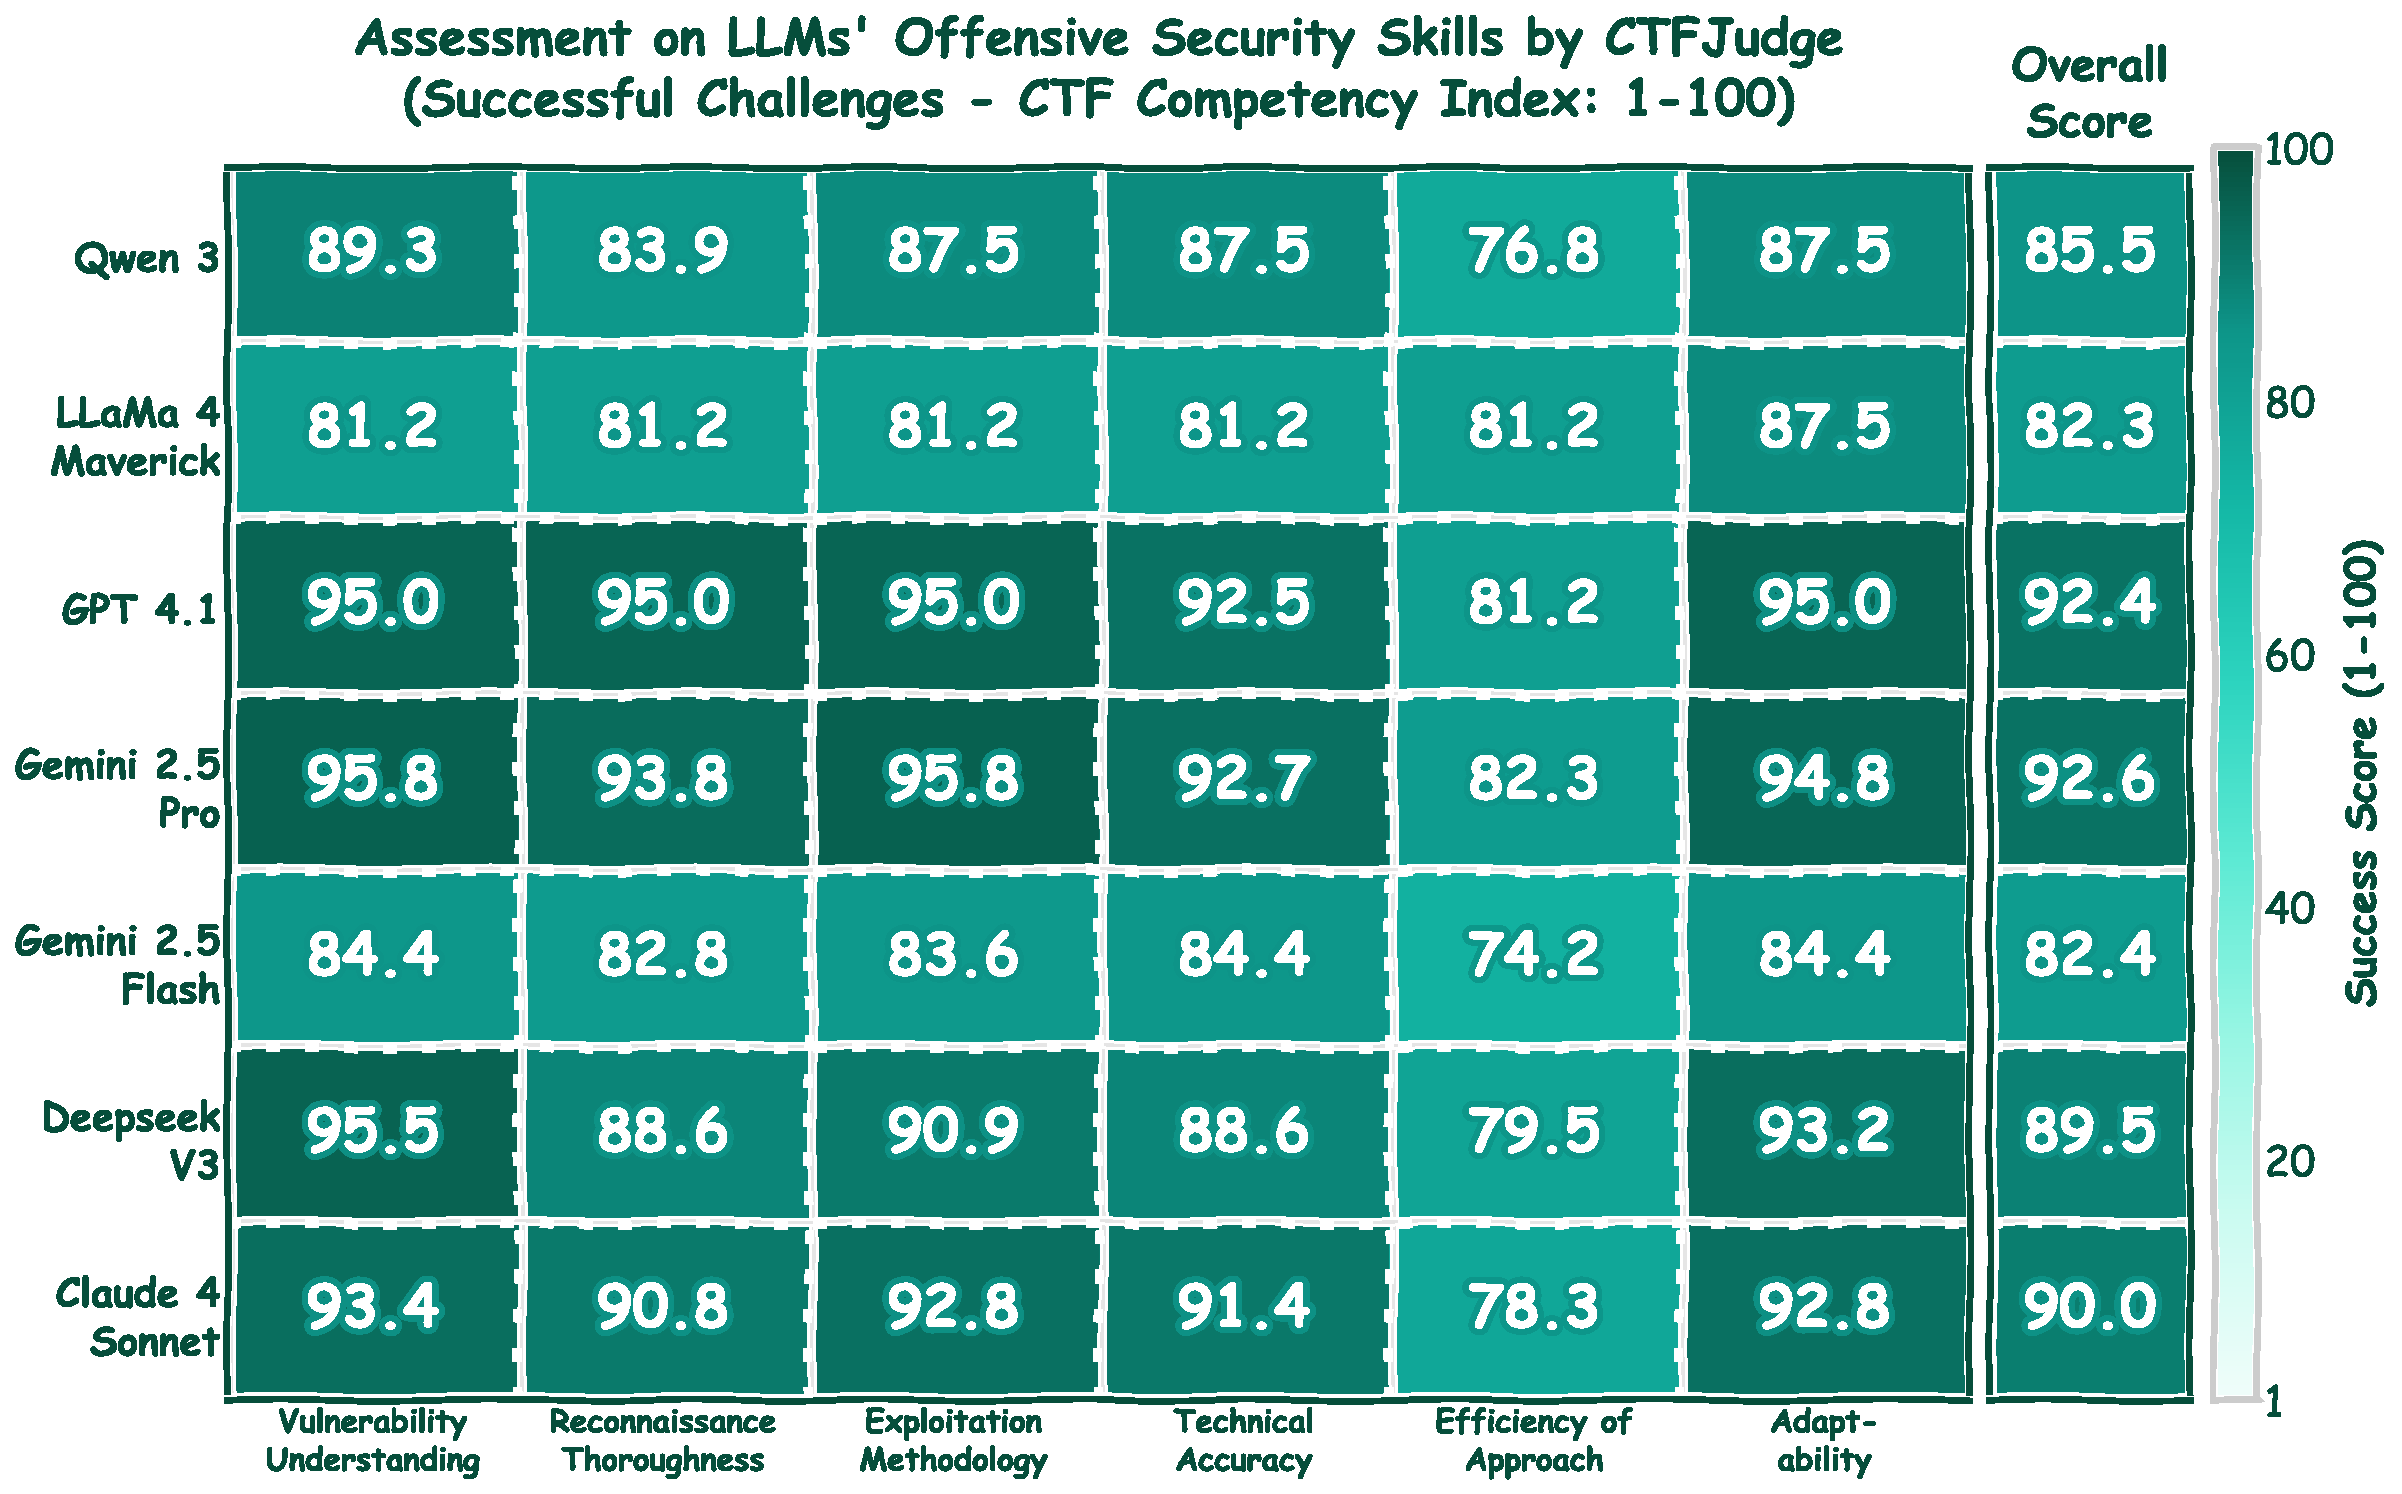
\includegraphics[width=1.1\linewidth]{diagrams/ctfjudge_success_result.pdf}
    \caption{CTF Competency Index on a succeedsful solution.} %, high solve rates don’t always mean better reasoning.}
    \label{fig:cci_succ}
\end{figure}

Key observations reinforce these patterns: Gemini 2.5 Pro, while solving fewer challenges than Flash, achieves higher average CCI, especially in exploitation and adaptability, suggesting more structured, human-aligned reasoning. Most models underperform on "Efficiency of Approach", relying on brute-force or redundant exploration---a clear bottleneck under cost constraints. CCI exposes the gap between solve rates and true reasoning quality, showing brute-force success rarely translates to robust, interpretable agent behavior. These findings highlight the need to evaluate agents by structured reasoning and operational efficiency, not solve count.

\begin{figure}[!b]\
\hspace*{-0.15in}
    \centering
    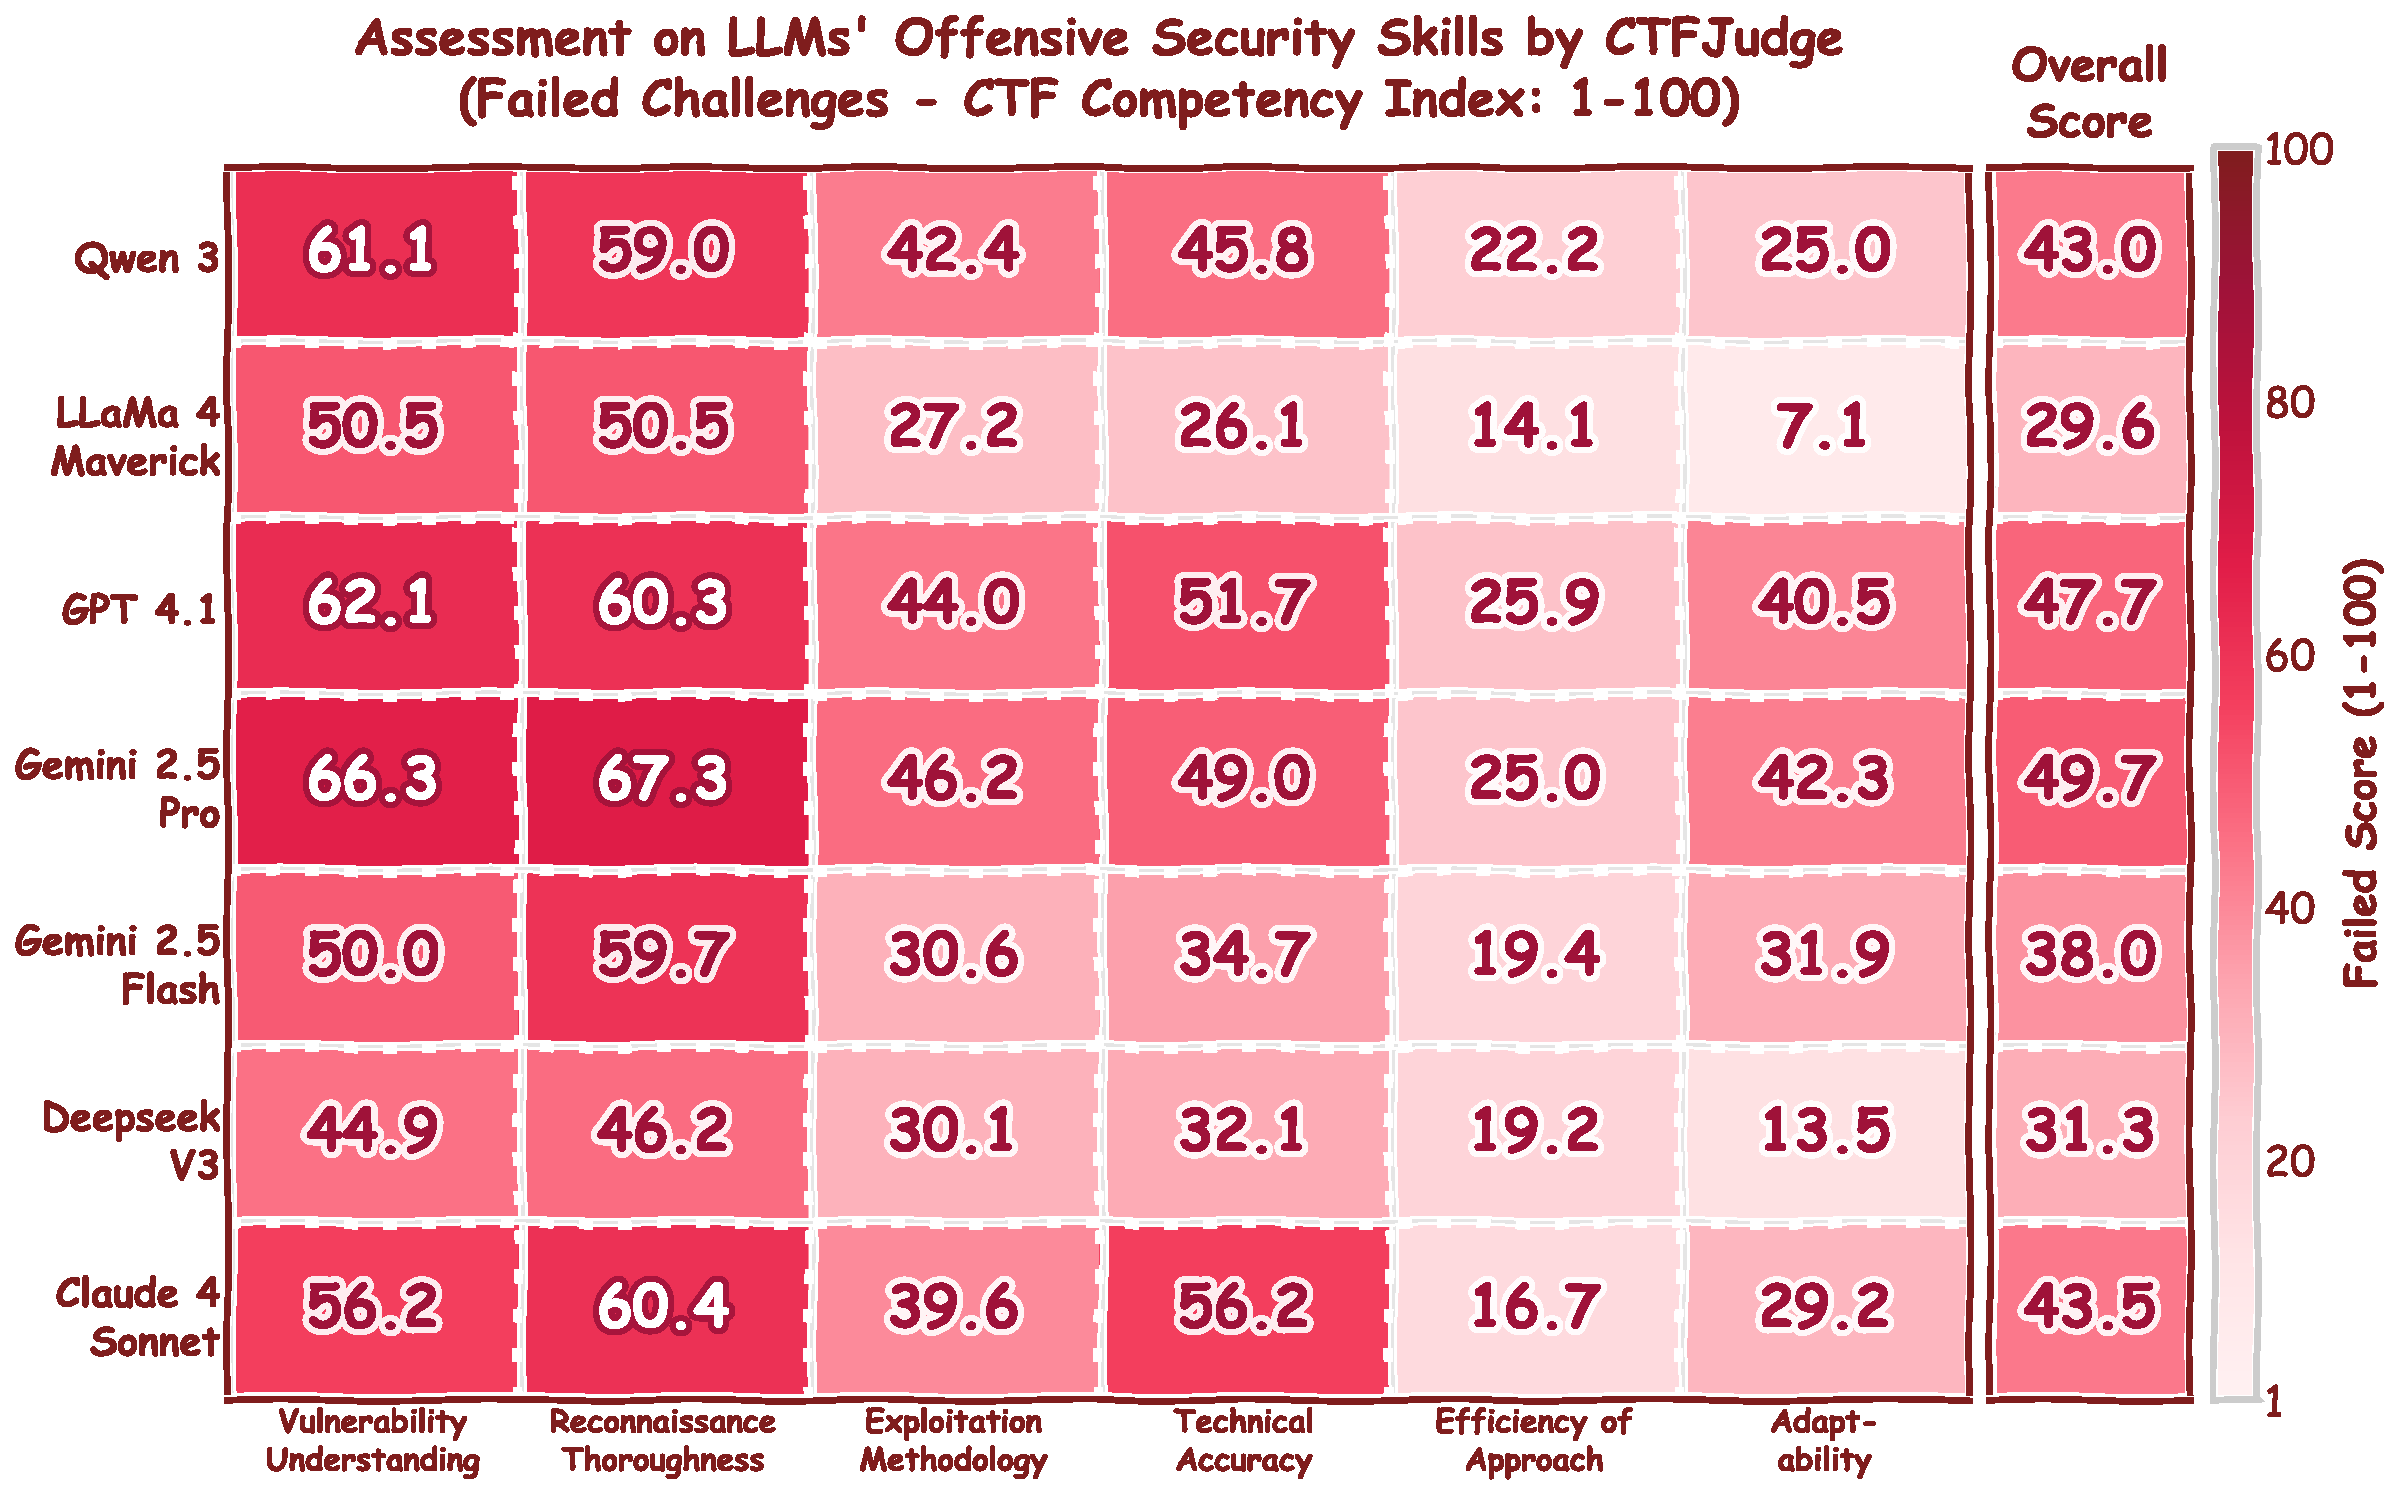
\includegraphics[width=1.1\linewidth]{diagrams/ctfjudge_failed_result.pdf}
    \caption{CTF Competency Index on failed solution.} %, high solve rates don’t always mean better reasoning.}
    \label{fig:cci_fail}
\end{figure}



Figure~\ref{fig:cci_category} compares CCI by category. Claude 4 Sonnet is the most balanced; Gemini 2.5 Pro is similar with peaks in \textbf{for} and \textbf{pwn}. Flash excels in \textbf{for} and \textbf{web} but dips on \textbf{rev} and \textbf{msc}. GPT-4.1 spikes on web; Qwen 3 is mid-tier; DeepSeek V3 and LLaMA-4 Maverick remain low. Notably, \textbf{misc} and \textbf{pwn} show lower CCI, likely due to heavier reliance on challenge-server interaction, which adds overhead and fragility and lowers Efficiency/Adaptability relative to categories that rely more on local environments such as \textbf{rev}. \textbf{for} also lags, plausibly because challenges require handling diverse file types, which remains difficult for LLMs. \textbf{web} and \textbf{cry} score higher as their challenge formats are more standardized and pattern-repetitive, easing reasoning and verification under fixed toolchains and protocols.

\begin{figure}[t!]
    \centering
    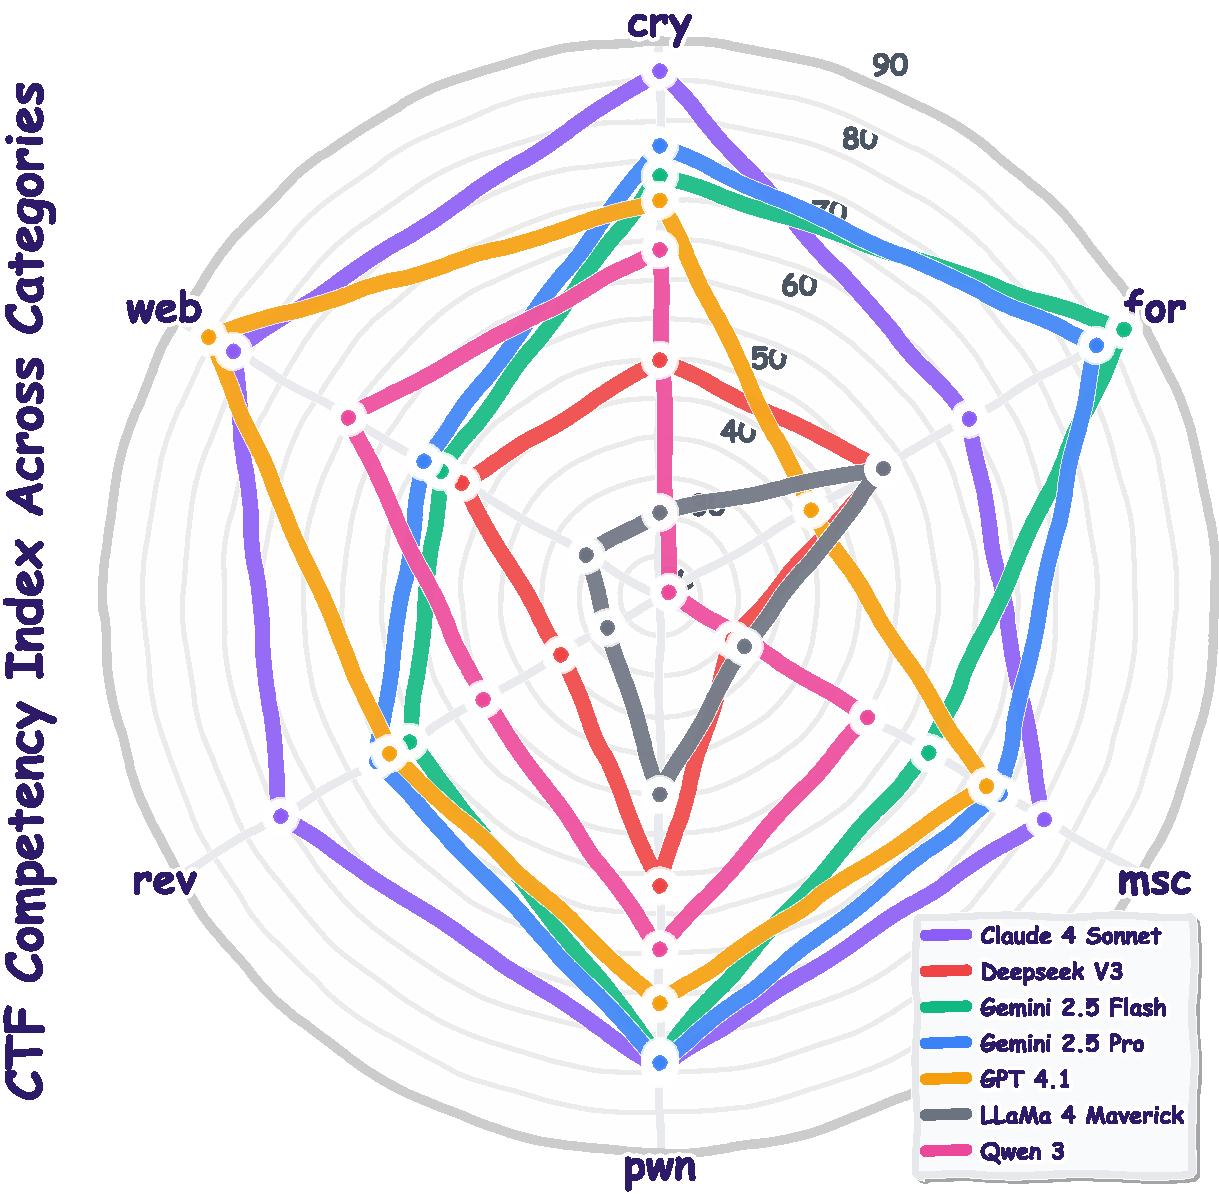
\includegraphics[width=0.8\linewidth]{diagrams/ctfjudge_category_radar.pdf}
    \caption{Category-wise CTF Competency Index across models, highlighting misc, pwn, and forensics challenges.} %, high solve rates don’t always mean better reasoning.}
    \label{fig:cci_category}
\end{figure}
\subsection{Impact of Hyperparameters}

We systematically analyze how temperature, top-p, and maximum token length affect LLM-based CTF agent performance, revealing their roles in shaping reasoning stability, execution precision, and success across diverse challenge types.

\begin{figure}[htbp]
    \centering
    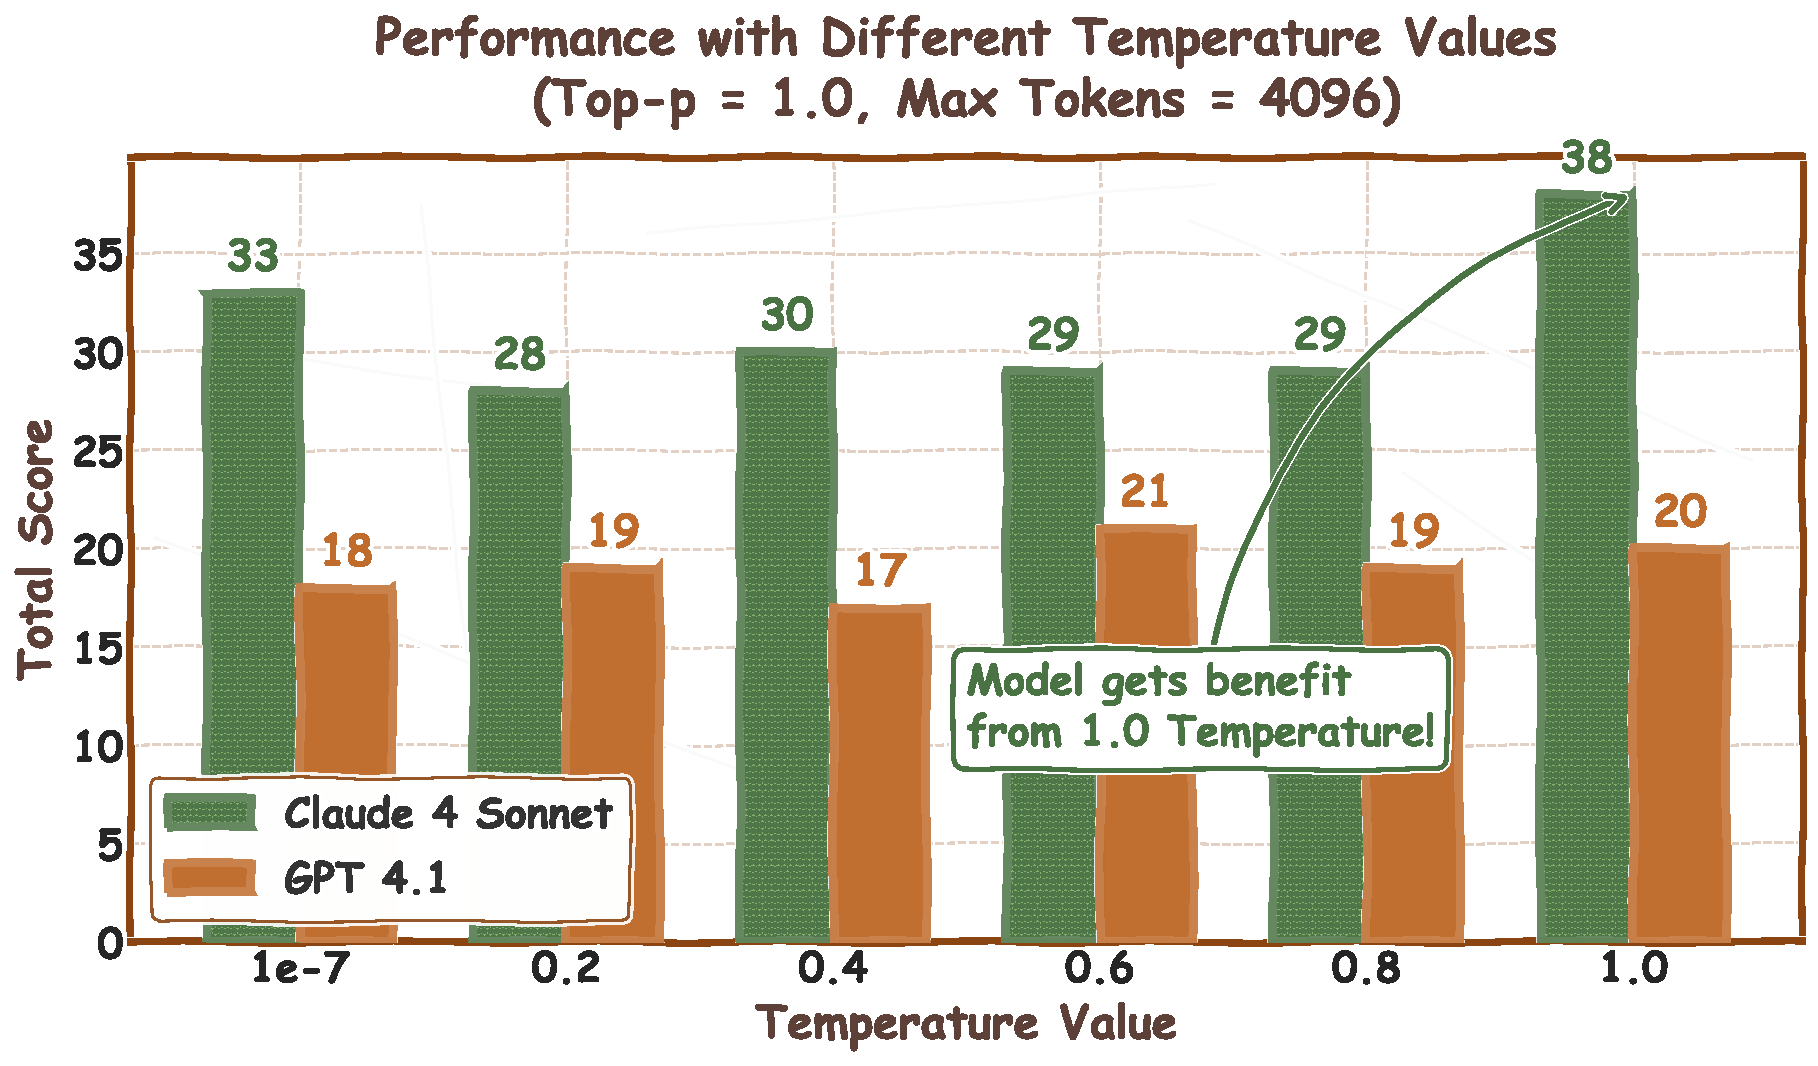
\includegraphics[width=\linewidth]{diagrams/temperature_sweep.pdf}
    \caption{Model accuracy peaks at high temperature, highlighting the need for creative reasoning.}
    \label{fig:temp_sweep}
\end{figure}


\subsubsection{Temperature.} As shown in Figure~\ref{fig:temp_sweep}, model performance exhibits non-linear relationship with temperature. \texttt{Claude 4 Sonnet} reaches peak accuracy at the highest value ($T = 1.0$) with 38 correct solves, contrasting with lower performance at intermediate settings. This suggests that controlled randomness enhances exploratory reasoning, especially in open-ended challenges. Claude’s performance remains stable across $T \in [0.2, 0.8]$, then surges at $T = 1.0$, pointing to creative reasoning benefits under high-temperature sampling. In contrast, \texttt{GPT-4.1} peaks at $T = 0.6$ (21 solves), with minimal variance across the sweep, indicating conservative decoding that resists both gains and drops. Overall, high temperature appears advantageous for models that effectively leverage generative diversity, particularly in ambiguous or multi-path problems common in CTF tasks.

\begin{figure}[htbp]
    \centering
    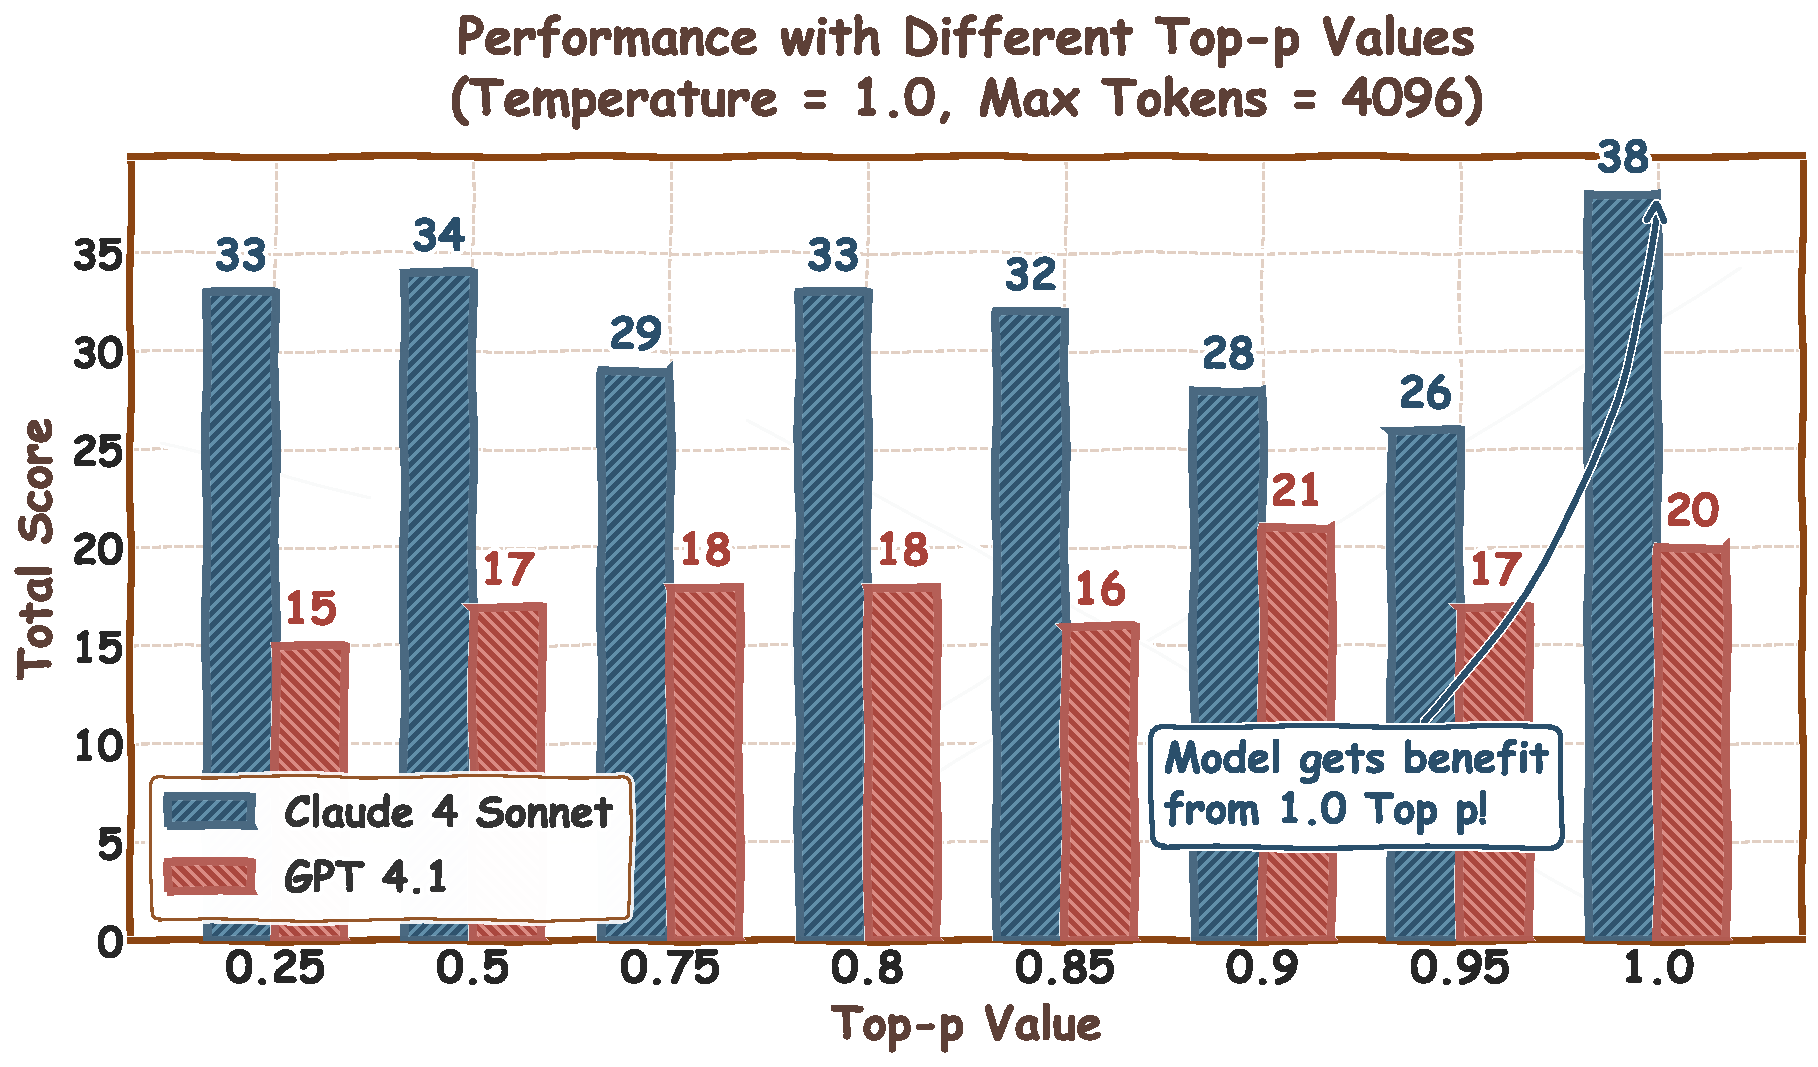
\includegraphics[width=\linewidth]{diagrams/topp_sweep.pdf}
    \caption{Model performance is stable across most top-p, with only the highest top-p  notably increasing solve rates.}
    \label{fig:topp_sweep}
\end{figure}

\subsubsection{Top-$p$.} In contrast to temperature, top-$p$ adjusts diversity by truncating the token distribution. As shown in Figure~\ref{fig:topp_sweep}, Claude 4 Sonnet performs consistently across $p \in [0.25, 0.85]$, hovering around 32–34 solves, and peaks at $p=1.0$ with 38 solves—suggesting full distributional access can boost exploration in strong models. This challenges the notion that lower top-p harms performance via distractor tokens. While minor fluctuations appear, Claude’s robustness implies control over long-tail generations. In contrast, \texttt{GPT-4.1} performs stably between $p = 0.75$ and $0.9$, peaking modestly at $p=0.9$ with 21 solves, and shows no major drop at $p=1.0$. These findings suggest that top-p near 1.0 may benefit models able to leverage expanded output space, especially in creative or underspecified CTF tasks.

\begin{figure}[htbp]
    \centering
    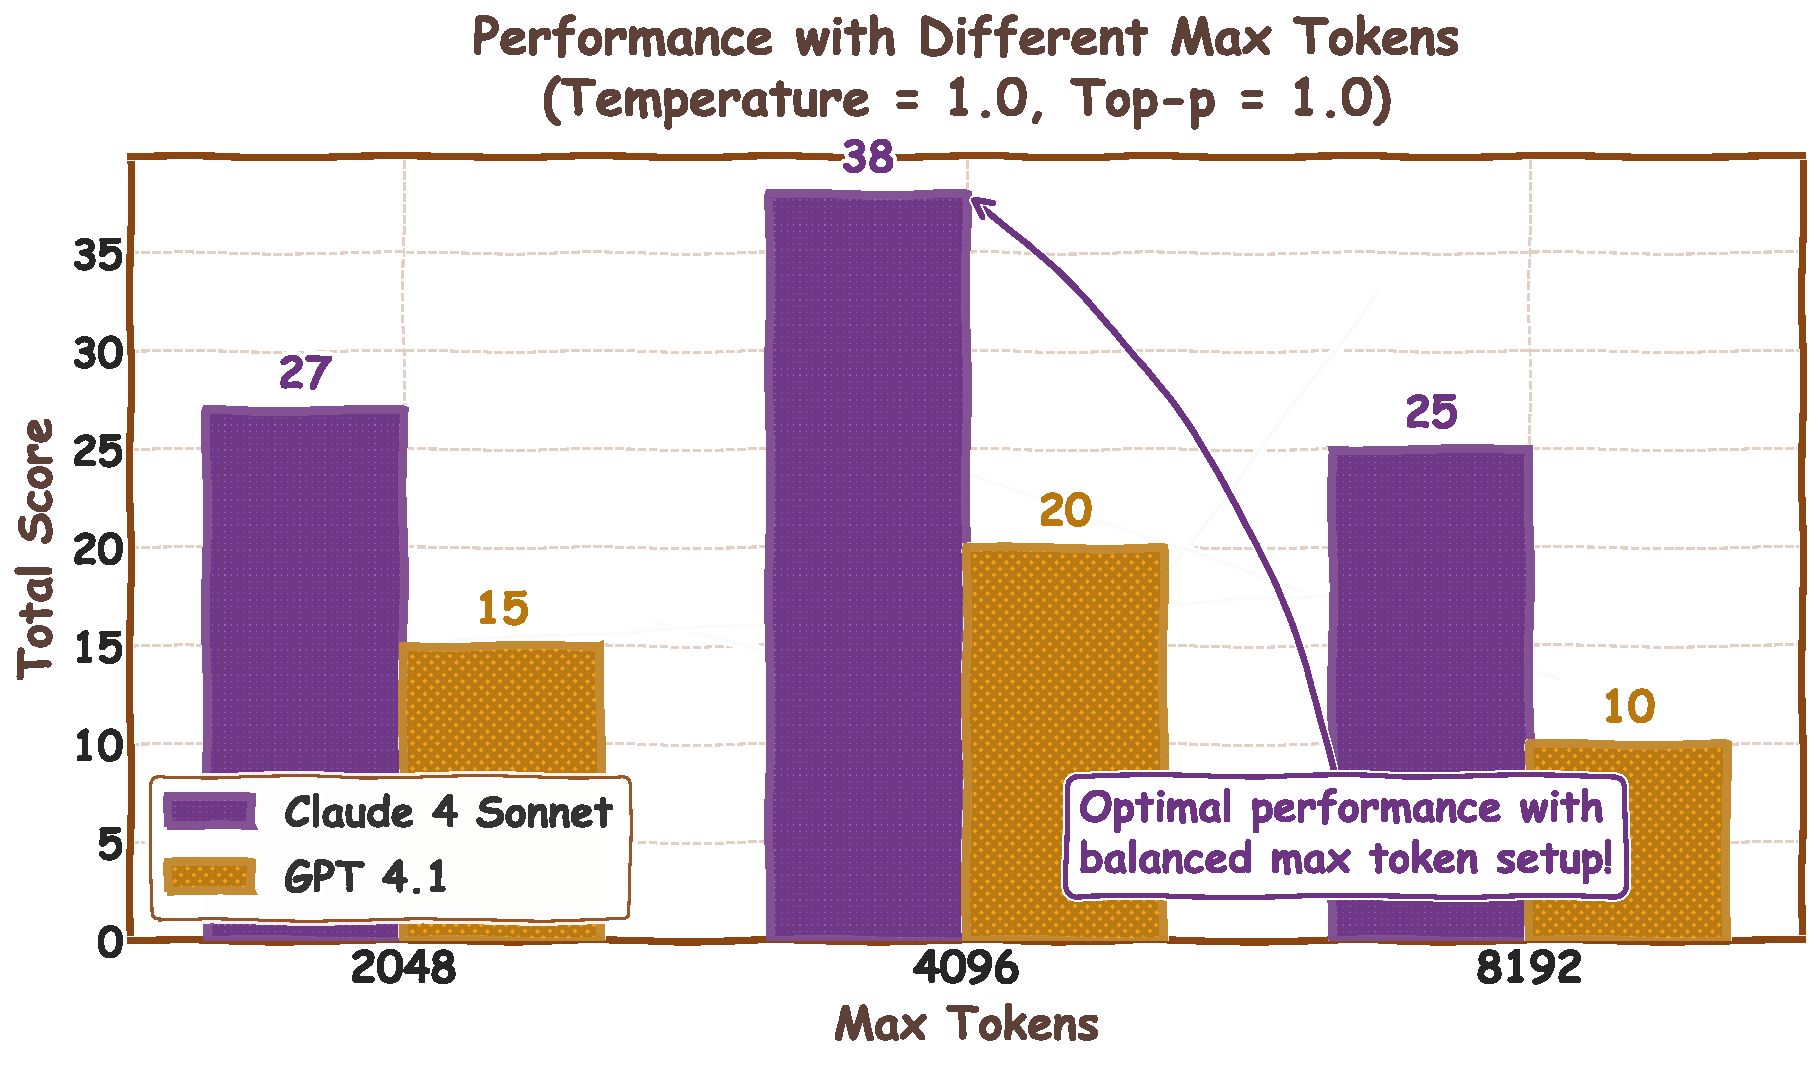
\includegraphics[width=\linewidth]{diagrams/max_token_sweep.pdf}
    \caption{Mid-range max tokens yield best accuracy, while shorter or longer contexts hurt performance.}
    \label{fig:max_token_sweep}
\end{figure}

\textbf{Max Tokens}. Figure~\ref{fig:max_token_sweep} presents a counterintuitive finding: longer context windows do not always improve performance. Claude 4 Sonnet peaks at 4096 tokens, solving 38 challenges, while performance drops at both 2048 and 8192. The dip at 8192 suggests context saturation, where longer completions may overwhelm model’s attention or generate overly verbose. This is especially problematic when prompt grounding is critical for correct planning, such as in \textbf{pwn} or \textbf{rev}. GPT-4.1 mirrors this trend with a modest peak at 4096 (20 solves), dropping to 10 at 8192. These results highlight a “Goldilocks zone” for context size: large enough to support complex reasoning, but not so large as to induce distraction or drift.

Taken together, these results show that model behavior is sensitive to decoding configurations, and optimal settings require balancing determinism with exploration. Our study finds that higher temperature ($\approx$ 1.0) and top-p ($\approx$ 1.0) improve solve rates, particularly for strong models like Claude, by enabling flexible, multi-step reasoning. Low temperature, moderate top-p, and mid-range token lengths (4096) still offer a favorable trade-off between accuracy, stability, and efficiency, especially in precision-heavy domains. Though not universally optimal, these configurations form a strong baseline for LLM-based cybersecurity agents, with tuning informed by task complexity and feedback.


\subsection{Failure Analysis}
% \nanda{TODO, write the text part}

We conducted a detailed analysis of model failures using $21$ predefined categories highly relevant to cyber and agentic deficiencies. For each unsolved challenge the \texttt{CTFJudge} framework identified one or more reasons for failure and extracted key terms reflecting the root cause. Depending on the agent's reasoning trace each unsolved challenge could be associated with multiple reasons for failure.The overall distribution of these failure types is presented in the line graph in Fig~\ref{fig:failure_analysis}. The most frequent reason observed was a `Knowledge or Domain Expertise Gap', followed by `Exploit Development Failure' and `Insufficient Reconnaissance.' These findings suggest models struggle due to limited understanding of CTF skills, inability to translate vulnerabilities into exploits, or failure to gather necessary scenario information. Notably despite \texttt{D-CIPHER} being a coordinated agentic framework, "Incorrect Task Delegation" and "Infrastructure or Environment Failure:" were in the lowest quartile for failures. 

We performed a model-wise failure breakdown, shown in the heatmap\footnote{Y-axis of heatmap shows failure reasons in the line graph.} in Fig~\ref{fig:failure_analysis}. LLaMa 4 Maverick showed the highest failure rates, while Claude 4 Sonnet had the lowest. The columns reveal a gradient: weaker models (LLaMa 4 Maverick, Qwen 3, DeepSeek V3) accumulate more failures; stronger ones (Claude 4 Sonnet, Gemini 2.5 Pro/Flash) show fewer, more concentrated errors. Gemini 2.5 Pro and Flash fall in between, matching their mid-tier solve counts. Except for Claude, all models show a steep drop from high to low frequency failure reasons, while Claude maintains uniformly low counts, indicating robustness. Overall, failure volume inversely tracks pass rate—better-performing models make fewer, less diffuse mistakes.

\begin{figure}[htbp]
    \hspace*{-0.15in}
    \centering
    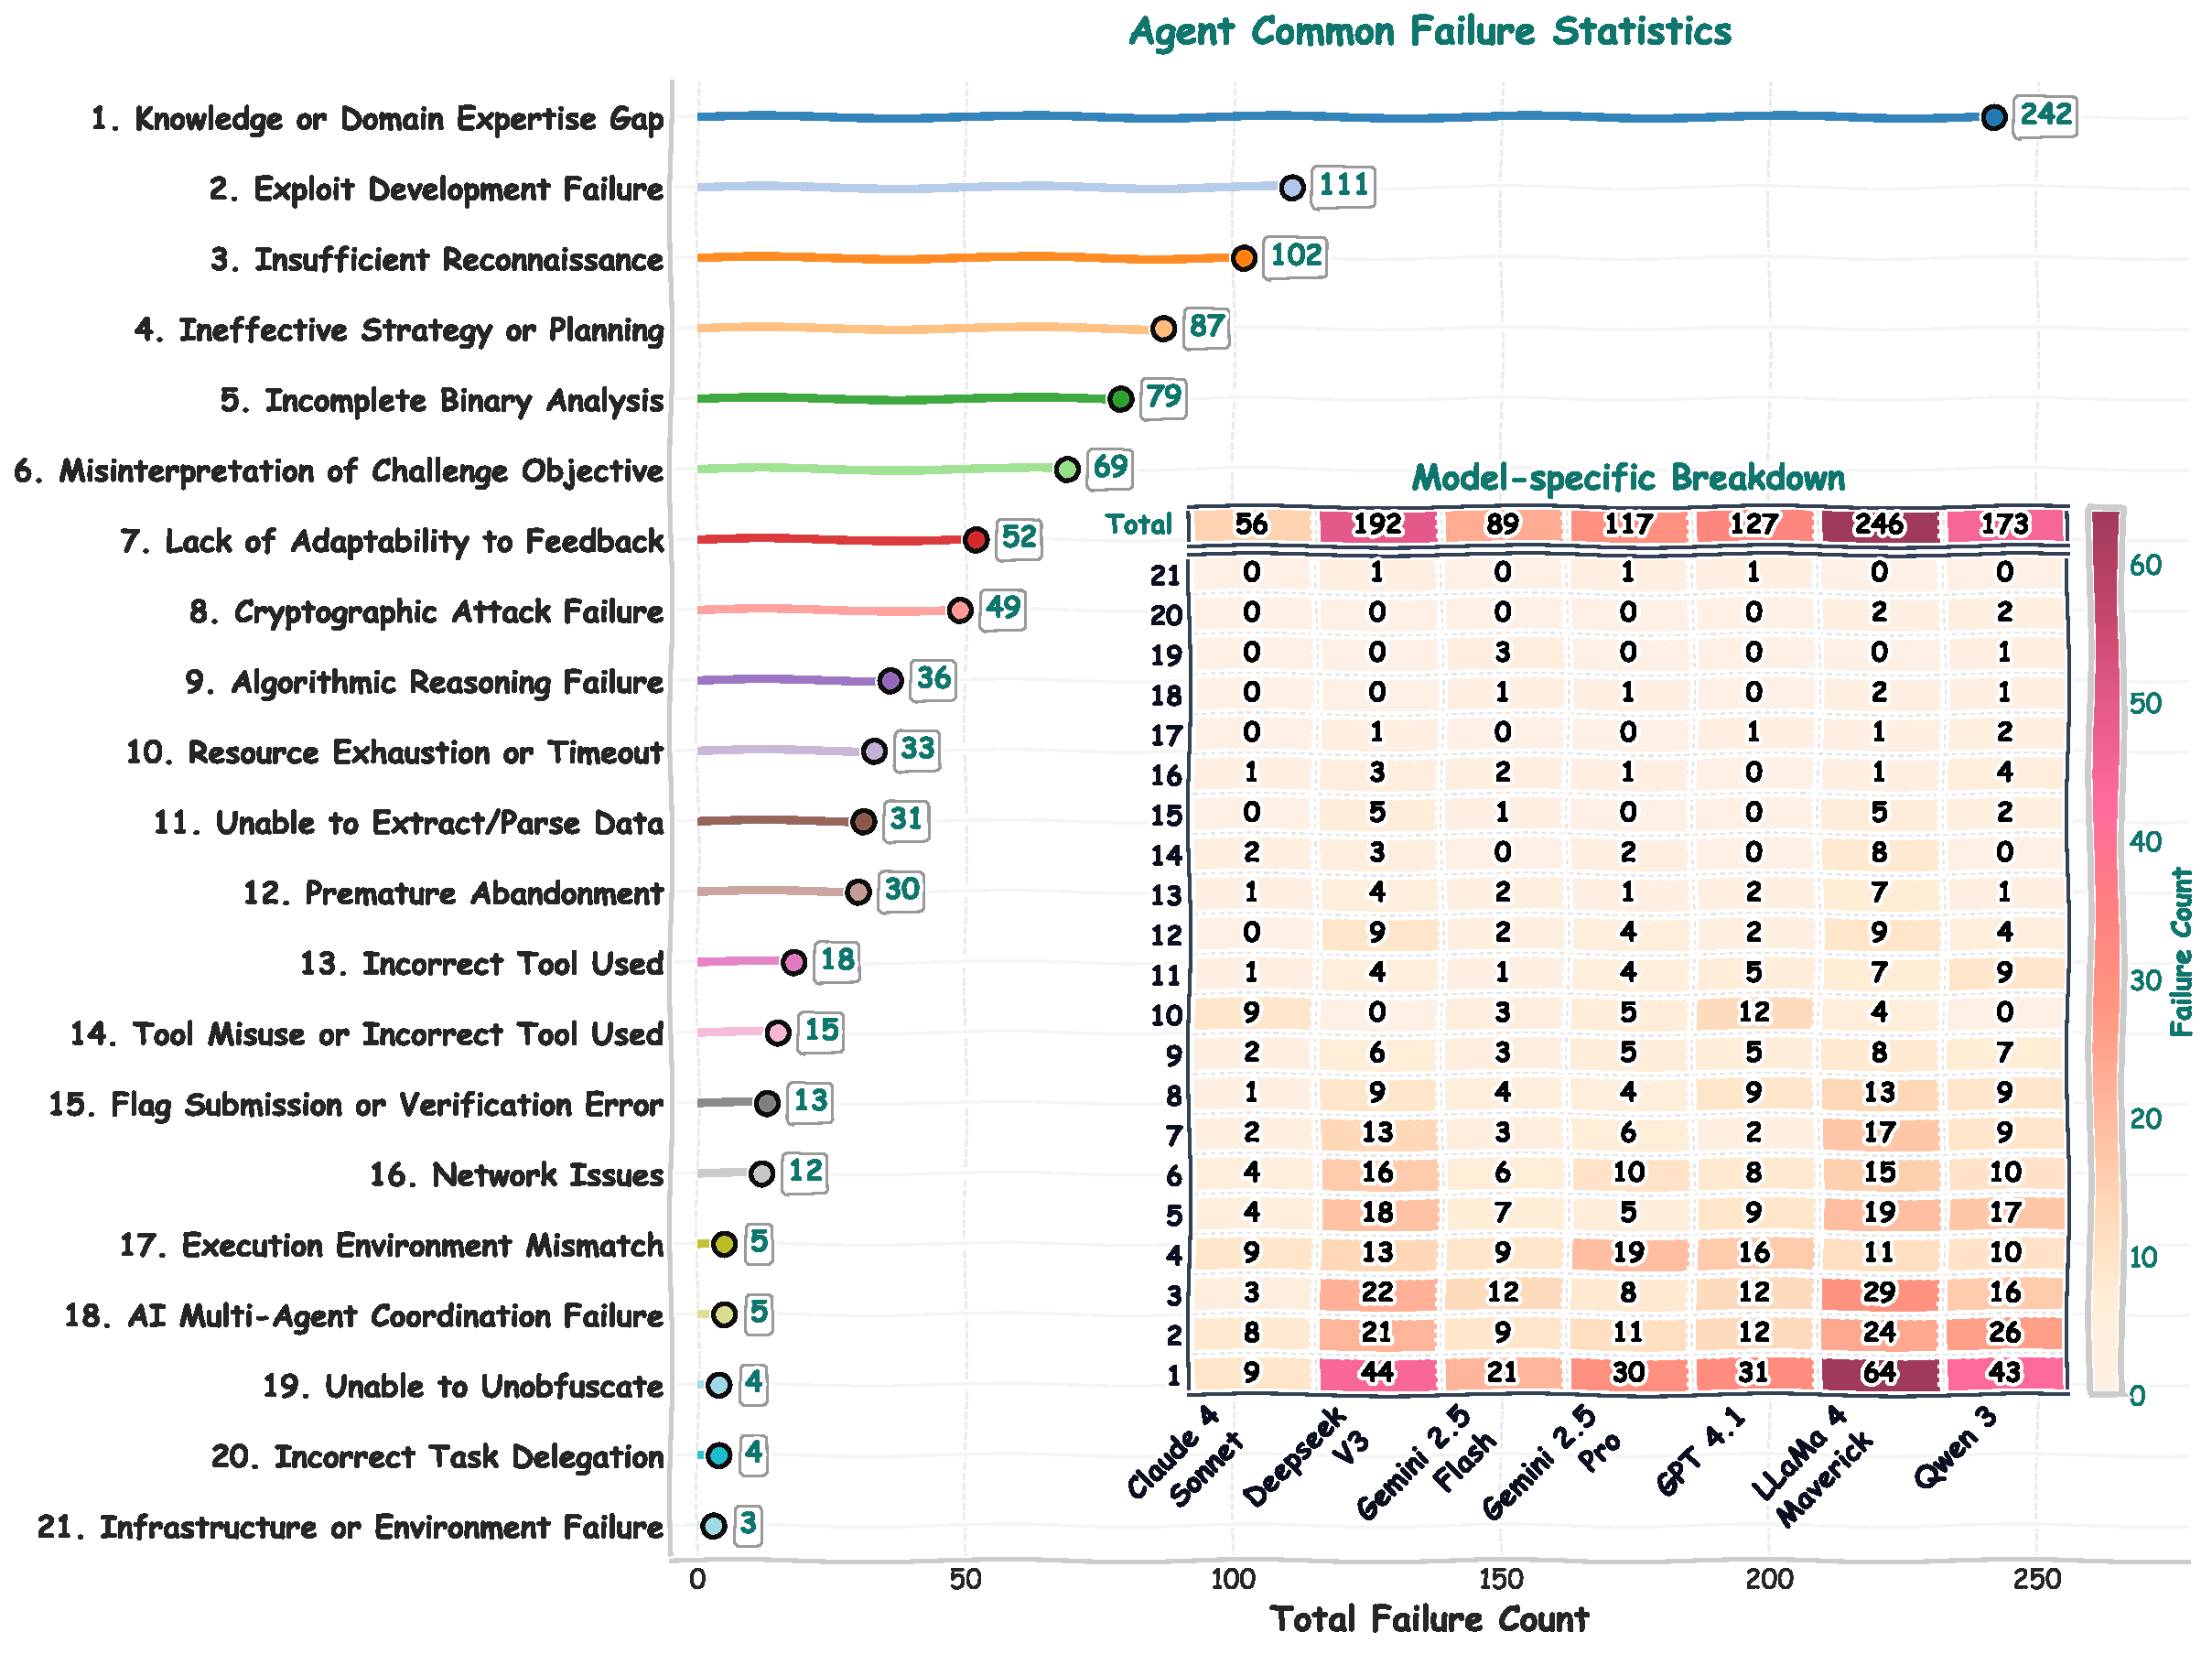
\includegraphics[width=1.1\linewidth]{diagrams/failure_analysis.pdf}
    \caption{Failure analysis shows domain knowledge and exploit development as main agent bottlenecks.}
    \label{fig:failure_analysis}
\end{figure}

% \begin{table*}[]
%     \centering
%     \begin{tabular}{lcccccccccc}
%     Model & Temp & TopP & Q1 & Q2 & Q3 & Q4 & Q5 & Q6 & Q7 & Q8\\
%     \midrule
% Claude 4 Sonnet & 0.0 & 1.00 & \cellcolor{blue!5}{0.05} & \cellcolor{blue!15}{0.15} & \cellcolor{blue!17}{0.17} & \cellcolor{blue!21}{0.21} & \cellcolor{blue!21}{0.21} & \cellcolor{blue!23}{0.23} & \cellcolor{blue!33}{0.33} & \cellcolor{blue!63}{0.63} \\
% Claude 4 Sonnet & 0.2 & 1.00 & \cellcolor{blue!2}{0.02} & \cellcolor{blue!15}{0.15} & \cellcolor{blue!15}{0.15} & \cellcolor{blue!18}{0.18} & \cellcolor{blue!15}{0.15} & \cellcolor{blue!24}{0.24} & \cellcolor{blue!18}{0.18} & \cellcolor{blue!58}{0.58} \\
% Claude 4 Sonnet & 0.4 & 1.00 & \cellcolor{blue!3}{0.03} & \cellcolor{blue!10}{0.10} & \cellcolor{blue!16}{0.16} & \cellcolor{blue!17}{0.17} & \cellcolor{blue!18}{0.18} & \cellcolor{blue!30}{0.30} & \cellcolor{blue!28}{0.28} & \cellcolor{blue!51}{0.51} \\
% Claude 4 Sonnet & 0.6 & 1.00 & \cellcolor{blue!3}{0.03} & \cellcolor{blue!13}{0.13} & \cellcolor{blue!24}{0.24} & \cellcolor{blue!19}{0.19} & \cellcolor{blue!18}{0.18} & \cellcolor{blue!29}{0.29} & \cellcolor{blue!31}{0.31} & \cellcolor{blue!71}{0.71} \\
% Claude 4 Sonnet & 0.8 & 1.00 & \cellcolor{blue!2}{0.02} & \cellcolor{blue!25}{0.25} & \cellcolor{blue!14}{0.14} & \cellcolor{blue!9}{0.09} & \cellcolor{blue!21}{0.21} & \cellcolor{blue!25}{0.25} & \cellcolor{blue!36}{0.36} & \cellcolor{blue!64}{0.64} \\
% Claude 4 Sonnet & 1.0 & 0.25 & \cellcolor{blue!4}{0.04} & \cellcolor{blue!7}{0.07} & \cellcolor{blue!29}{0.29} & \cellcolor{blue!16}{0.16} & \cellcolor{blue!23}{0.23} & \cellcolor{blue!21}{0.21} & \cellcolor{blue!24}{0.24} & \cellcolor{blue!45}{0.45} \\
% Claude 4 Sonnet & 1.0 & 0.50 & \cellcolor{blue!3}{0.03} & \cellcolor{blue!13}{0.13} & \cellcolor{blue!18}{0.18} & \cellcolor{blue!23}{0.23} & \cellcolor{blue!27}{0.27} & \cellcolor{blue!26}{0.26} & \cellcolor{blue!28}{0.28} & \cellcolor{blue!51}{0.51} \\
% Claude 4 Sonnet & 1.0 & 0.75 & \cellcolor{blue!7}{0.07} & \cellcolor{blue!14}{0.14} & \cellcolor{blue!17}{0.17} & \cellcolor{blue!22}{0.22} & \cellcolor{blue!18}{0.18} & \cellcolor{blue!32}{0.32} & \cellcolor{blue!32}{0.32} & \cellcolor{blue!55}{0.55} \\
% Claude 4 Sonnet & 1.0 & 1.00 & \cellcolor{blue!7}{0.07} & \cellcolor{blue!10}{0.10} & \cellcolor{blue!16}{0.16} & \cellcolor{blue!26}{0.26} & \cellcolor{blue!25}{0.25} & \cellcolor{blue!31}{0.31} & \cellcolor{blue!37}{0.37} & \cellcolor{blue!62}{0.62} \\
% DeepSeek V3 & 1.0 & 1.00 & \cellcolor{blue!4}{0.04} & \cellcolor{blue!17}{0.17} & \cellcolor{blue!18}{0.18} & \cellcolor{blue!14}{0.14} & \cellcolor{blue!27}{0.27} & \cellcolor{blue!23}{0.23} & \cellcolor{blue!25}{0.25} & \cellcolor{blue!42}{0.42} \\
% GPT 4.1 & 0.0 & 1.00 & \cellcolor{blue!13}{0.13} & \cellcolor{blue!20}{0.20} & \cellcolor{blue!19}{0.19} & \cellcolor{blue!31}{0.31} & \cellcolor{blue!22}{0.22} & \cellcolor{blue!22}{0.22} & \cellcolor{blue!16}{0.16} & \cellcolor{blue!37}{0.37} \\
% GPT 4.1 & 0.2 & 1.00 & \cellcolor{blue!8}{0.08} & \cellcolor{blue!25}{0.25} & \cellcolor{blue!19}{0.19} & \cellcolor{blue!20}{0.20} & \cellcolor{blue!22}{0.22} & \cellcolor{blue!19}{0.19} & \cellcolor{blue!19}{0.19} & \cellcolor{blue!30}{0.30} \\
% GPT 4.1 & 0.4 & 1.00 & \cellcolor{blue!0}{0.00} & \cellcolor{blue!5}{0.05} & \cellcolor{blue!4}{0.04} & \cellcolor{blue!25}{0.25} & \cellcolor{blue!19}{0.19} & \cellcolor{blue!8}{0.08} & \cellcolor{blue!8}{0.08} & \cellcolor{blue!21}{0.21} \\
% GPT 4.1 & 0.6 & 1.00 & \cellcolor{blue!9}{0.09} & \cellcolor{blue!15}{0.15} & \cellcolor{blue!25}{0.25} & \cellcolor{blue!18}{0.18} & \cellcolor{blue!25}{0.25} & \cellcolor{blue!22}{0.22} & \cellcolor{blue!21}{0.21} & \cellcolor{blue!31}{0.31} \\
% GPT 4.1 & 0.8 & 1.00 & \cellcolor{blue!9}{0.09} & \cellcolor{blue!12}{0.12} & \cellcolor{blue!16}{0.16} & \cellcolor{blue!5}{0.05} & \cellcolor{blue!18}{0.18} & \cellcolor{blue!17}{0.17} & \cellcolor{blue!25}{0.25} & \cellcolor{blue!34}{0.34} \\
% GPT 4.1 & 1.0 & 0.25 & \cellcolor{blue!10}{0.10} & \cellcolor{blue!13}{0.13} & \cellcolor{blue!24}{0.24} & \cellcolor{blue!20}{0.20} & \cellcolor{blue!16}{0.16} & \cellcolor{blue!19}{0.19} & \cellcolor{blue!27}{0.27} & \cellcolor{blue!35}{0.35} \\
% GPT 4.1 & 1.0 & 0.50 & \cellcolor{blue!7}{0.07} & \cellcolor{blue!10}{0.10} & \cellcolor{blue!23}{0.23} & \cellcolor{blue!25}{0.25} & \cellcolor{blue!14}{0.14} & \cellcolor{blue!15}{0.15} & \cellcolor{blue!29}{0.29} & \cellcolor{blue!38}{0.38} \\
% GPT 4.1 & 1.0 & 0.75 & \cellcolor{blue!5}{0.05} & \cellcolor{blue!4}{0.04} & \cellcolor{blue!11}{0.11} & \cellcolor{blue!6}{0.06} & \cellcolor{blue!4}{0.04} & \cellcolor{blue!5}{0.05} & \cellcolor{blue!3}{0.03} & \cellcolor{blue!22}{0.22} \\
% GPT 4.1 & 1.0 & 1.00 & \cellcolor{blue!8}{0.08} & \cellcolor{blue!11}{0.11} & \cellcolor{blue!14}{0.14} & \cellcolor{blue!25}{0.25} & \cellcolor{blue!11}{0.11} & \cellcolor{blue!25}{0.25} & \cellcolor{blue!17}{0.17} & \cellcolor{blue!35}{0.35} \\
% LLaMa 4 Maverick & 1.0 & 1.00 & \cellcolor{blue!17}{0.17} & \cellcolor{blue!12}{0.12} & \cellcolor{blue!0}{0.00} & \cellcolor{blue!75}{0.75} & \cellcolor{blue!38}{0.38} & \cellcolor{blue!12}{0.12} & \cellcolor{blue!25}{0.25} & \cellcolor{blue!50}{0.50} \\
% Qwen 3 & 1.0 & 1.00 & \cellcolor{blue!16}{0.16} & \cellcolor{blue!14}{0.14} & \cellcolor{blue!29}{0.29} & \cellcolor{blue!36}{0.36} & \cellcolor{blue!42}{0.42} & \cellcolor{blue!18}{0.18} & \cellcolor{blue!9}{0.09} & \cellcolor{blue!35}{0.35} \\
%     \end{tabular}
%     \caption{Caption}
%     \label{tab:my_label}
% \end{table*}

% \begin{table*}[]
%     \centering
%     \begin{tabular}{lcccccccccc}
%     Model & Temp & TopP & Q1 & Q2 & Q3 & Q4 & Q5 & Q6 & Q7 & Q8 \\
%     \midrule
% Claude 4 Sonnet & 0.0 & 1.00 & \cellcolor{red!5}{-0.07} & \cellcolor{red!6}{-0.09} & \cellcolor{red!10}{-0.14} & \cellcolor{red!12}{-0.17} & \cellcolor{red!18}{-0.26} & \cellcolor{red!9}{-0.13} & \cellcolor{red!0}{-0.01} & \cellcolor{blue!21}{0.31} \\
% Claude 4 Sonnet & 0.2 & 1.00 & \cellcolor{red!10}{-0.14} & \cellcolor{blue!11}{0.15} & \cellcolor{red!8}{-0.11} & \cellcolor{red!14}{-0.20} & \cellcolor{red!16}{-0.23} & \cellcolor{red!6}{-0.08} & \cellcolor{red!12}{-0.16} & \cellcolor{blue!20}{0.29} \\
% Claude 4 Sonnet & 0.4 & 1.00 & \cellcolor{red!10}{-0.14} & \cellcolor{red!20}{-0.29} & \cellcolor{red!12}{-0.17} & \cellcolor{red!8}{-0.12} & \cellcolor{red!22}{-0.32} & \cellcolor{red!12}{-0.17} & \cellcolor{red!16}{-0.22} & \cellcolor{blue!12}{0.16} \\
% Claude 4 Sonnet & 0.6 & 1.00 & \cellcolor{red!8}{-0.12} & \cellcolor{blue!5}{0.08} & \cellcolor{blue!0}{0.01} & \cellcolor{red!8}{-0.12} & \cellcolor{red!11}{-0.16} & \cellcolor{red!5}{-0.07} & \cellcolor{red!3}{-0.04} & \cellcolor{blue!36}{0.52} \\
% Claude 4 Sonnet & 0.8 & 1.00 & \cellcolor{red!20}{-0.28} & \cellcolor{blue!12}{0.17} & \cellcolor{red!0}{-0.01} & \cellcolor{red!13}{-0.19} & \cellcolor{red!7}{-0.10} & \cellcolor{red!8}{-0.12} & \cellcolor{blue!1}{0.02} & \cellcolor{blue!24}{0.34} \\
% Claude 4 Sonnet & 1.0 & 0.25 & \cellcolor{red!12}{-0.18} & \cellcolor{red!19}{-0.27} & \cellcolor{blue!6}{0.09} & \cellcolor{red!9}{-0.13} & \cellcolor{red!8}{-0.12} & \cellcolor{red!7}{-0.10} & \cellcolor{red!13}{-0.19} & \cellcolor{blue!6}{0.08} \\
% Claude 4 Sonnet & 1.0 & 0.50 & \cellcolor{red!1}{-0.01} & \cellcolor{red!14}{-0.21} & \cellcolor{blue!1}{0.01} & \cellcolor{blue!6}{0.08} & \cellcolor{red!1}{-0.01} & \cellcolor{red!7}{-0.09} & \cellcolor{red!5}{-0.07} & \cellcolor{blue!17}{0.24} \\
% Claude 4 Sonnet & 1.0 & 0.75 & \cellcolor{blue!2}{0.03} & \cellcolor{red!9}{-0.12} & \cellcolor{red!7}{-0.11} & \cellcolor{red!4}{-0.06} & \cellcolor{red!15}{-0.21} & \cellcolor{red!1}{-0.01} & \cellcolor{red!5}{-0.07} & \cellcolor{blue!16}{0.22} \\
% Claude 4 Sonnet & 1.0 & 1.00 & \cellcolor{red!5}{-0.08} & \cellcolor{red!14}{-0.20} & \cellcolor{red!2}{-0.03} & \cellcolor{red!4}{-0.05} & \cellcolor{red!4}{-0.06} & \cellcolor{red!2}{-0.03} & \cellcolor{blue!1}{0.02} & \cellcolor{blue!10}{0.14} \\
% DeepSeek V3 & 1.0 & 1.00 & \cellcolor{blue!3}{0.04} & \cellcolor{blue!25}{0.35} & \cellcolor{blue!12}{0.17} & \cellcolor{blue!2}{0.03} & \cellcolor{blue!14}{0.21} & \cellcolor{blue!9}{0.13} & \cellcolor{blue!13}{0.18} & \cellcolor{blue!30}{0.43} \\
% GPT 4.1 & 0.0 & 1.00 & \cellcolor{blue!7}{0.09} & \cellcolor{blue!18}{0.26} & \cellcolor{blue!10}{0.15} & \cellcolor{blue!20}{0.29} & \cellcolor{blue!11}{0.16} & \cellcolor{blue!20}{0.28} & \cellcolor{blue!9}{0.13} & \cellcolor{blue!33}{0.47} \\
% GPT 4.1 & 0.2 & 1.00 & \cellcolor{red!4}{-0.05} & \cellcolor{blue!9}{0.13} & \cellcolor{red!1}{-0.01} & \cellcolor{blue!4}{0.06} & \cellcolor{blue!6}{0.08} & \cellcolor{red!1}{-0.01} & \cellcolor{blue!2}{0.03} & \cellcolor{blue!22}{0.32} \\
% GPT 4.1 & 0.4 & 1.00 & \cellcolor{red!22}{-0.31} & \cellcolor{red!8}{-0.11} & \cellcolor{red!10}{-0.15} & \cellcolor{blue!14}{0.20} & \cellcolor{blue!7}{0.10} & \cellcolor{red!8}{-0.12} & \cellcolor{red!8}{-0.11} & \cellcolor{blue!11}{0.16} \\
% GPT 4.1 & 0.6 & 1.00 & \cellcolor{blue!2}{0.02} & \cellcolor{blue!5}{0.07} & \cellcolor{blue!22}{0.31} & \cellcolor{blue!13}{0.19} & \cellcolor{blue!10}{0.14} & \cellcolor{blue!10}{0.14} & \cellcolor{blue!15}{0.22} & \cellcolor{blue!33}{0.47} \\
% GPT 4.1 & 0.8 & 1.00 & \cellcolor{blue!6}{0.09} & \cellcolor{blue!2}{0.03} & \cellcolor{blue!5}{0.08} & \cellcolor{red!13}{-0.19} & \cellcolor{blue!8}{0.11} & \cellcolor{blue!11}{0.16} & \cellcolor{blue!22}{0.32} & \cellcolor{blue!33}{0.47} \\
% GPT 4.1 & 1.0 & 0.25 & \cellcolor{blue!10}{0.14} & \cellcolor{blue!7}{0.10} & \cellcolor{blue!14}{0.20} & \cellcolor{blue!6}{0.08} & \cellcolor{blue!3}{0.05} & \cellcolor{blue!8}{0.12} & \cellcolor{blue!15}{0.22} & \cellcolor{blue!27}{0.38} \\
% GPT 4.1 & 1.0 & 0.50 & \cellcolor{blue!1}{0.01} & \cellcolor{blue!11}{0.16} & \cellcolor{blue!24}{0.34} & \cellcolor{blue!21}{0.30} & \cellcolor{blue!10}{0.14} & \cellcolor{blue!5}{0.08} & \cellcolor{blue!20}{0.29} & \cellcolor{blue!32}{0.46} \\
% GPT 4.1 & 1.0 & 0.75 & \cellcolor{red!7}{-0.10} & \cellcolor{red!13}{-0.19} & \cellcolor{red!4}{-0.06} & \cellcolor{red!14}{-0.21} & \cellcolor{red!15}{-0.21} & \cellcolor{red!15}{-0.21} & \cellcolor{red!18}{-0.26} & \cellcolor{blue!9}{0.13} \\
% GPT 4.1 & 1.0 & 1.00 & \cellcolor{blue!0}{0.00} & \cellcolor{blue!3}{0.05} & \cellcolor{blue!6}{0.09} & \cellcolor{blue!16}{0.24} & \cellcolor{red!5}{-0.07} & \cellcolor{blue!17}{0.24} & \cellcolor{blue!11}{0.16} & \cellcolor{blue!31}{0.44} \\
% LLaMa 4 Maverick & 1.0 & 1.00 & \cellcolor{blue!6}{0.09} & \cellcolor{red!2}{-0.03} & \cellcolor{red!10}{-0.14} & \cellcolor{blue!32}{0.46} & \cellcolor{blue!12}{0.18} & \cellcolor{blue!1}{0.01} & \cellcolor{blue!8}{0.11} & \cellcolor{blue!24}{0.34} \\
% Qwen 3 & 1.0 & 1.00 & \cellcolor{blue!7}{0.10} & \cellcolor{red!5}{-0.08} & \cellcolor{blue!3}{0.04} & \cellcolor{blue!6}{0.09} & \cellcolor{blue!7}{0.10} & \cellcolor{red!10}{-0.15} & \cellcolor{red!18}{-0.26} & \cellcolor{blue!3}{0.04} \\
%     \end{tabular}
%     \caption{Caption}
%     \label{tab:my_label}
% \end{table*}